\documentclass{article}

\usepackage[final]{neurips_2024}

\usepackage[utf8]{inputenc}
\usepackage[T1]{fontenc}
\usepackage{hyperref}
\usepackage{url}
\usepackage{booktabs}
\usepackage{amsfonts}
\usepackage{nicefrac}
\usepackage{microtype}
\usepackage{xcolor}
\usepackage{graphicx}
\usepackage{multirow}
\usepackage{array}
\usepackage{tabularx}
\usepackage{makecell}

\title{Improving Brand Visibility Across LLM Platforms:\\
A Multi-Model Study of Generative Engine Optimization}

\author{%
  Divit Pratap Singh \\
  Khoury College of Computer Sciences \\
  Northeastern University \\
  \texttt{singh.divit@northeastern.edu} \\
  \And
  Uday Sonawane \\
  Khoury College of Computer Sciences \\
  Northeastern University \\
  \texttt{sonawane.u@northeastern.edu} \\
  \And
  Shantanu Shashank Dharmadhikari \\
  Khoury College of Computer Sciences \\
  Northeastern University \\
  \texttt{dharmadhikari.s@northeastern.edu} \\
}

\begin{document}

\maketitle

\begin{abstract}
As AI-powered search tools increasingly replace traditional search engines for product discovery, businesses face a new challenge: understanding and influencing how large language models (LLMs) represent their brand. This paper presents a systematic, multi-model study of Generative Engine Optimization (GEO) — the practice of optimizing content so that a brand appears prominently in LLM-generated recommendations. We evaluate brand visibility across state-of-the-art LLMs (GPT-4o-mini, Llama 4 Maverick, Mistral Large, and DeepSeek V3.2) using 140 product recommendation queries across CRM software and project management tool categories. We find significant disparities in brand visibility: HubSpot achieves an 87.1\% mention rate while Copper achieves 0\%, both consistently across all models. We further show that RAG-augmented injection of \emph{neutral} brand content unexpectedly \emph{decreases} mention rates — a \textbf{context dilution effect} — while RAG injection with \emph{optimized} content (using KDD 2024 GEO strategies: statistics, expert quotations, source citations) dramatically increases visibility. Most strikingly, Copper rises from 0\% to 100\% mention rate under optimized RAG injection. To isolate content-driven effects from parametric knowledge, we introduce a pseudo-brand experiment: a completely fictional CRM brand (``NexaCRM'') with no LLM training data achieves a 50\% mention rate and ranks \#1 in all cases where it is mentioned, demonstrating that optimized RAG content can establish brand presence from zero.
\end{abstract}

\section{Introduction}

The way consumers discover products is undergoing a fundamental shift. Traditional search engines, which surface links ranked by relevance signals, are rapidly being supplemented or replaced by conversational AI tools — ChatGPT, Claude, Gemini, Perplexity — that synthesize recommendations directly. When a user asks ``What is the best CRM for a 20-person startup?'', the LLM's response immediately shapes purchasing intent, often without the user consulting any other source.

This shift creates a new optimization problem for businesses. In traditional search, companies could measure and improve their visibility through well-understood SEO practices. In LLM-based recommendation, the mechanisms are opaque: which brands surface, in what order, and why is determined by the model's parametric knowledge and any context injected at inference time. Companies like Profound (valued at \$1B) and Azoma have emerged specifically to address this gap commercially, yet the underlying research on what drives LLM brand visibility — and how to systematically improve it — remains in its early stages.

The foundational work by Aggarwal et al.~\cite{aggarwal2024geo} at ACM SIGKDD 2024 introduced the term Generative Engine Optimization (GEO) and demonstrated that targeted content modifications — adding expert quotations (+41\% visibility), statistical claims (+33\%), and source citations (+31\%) — can meaningfully shift how often a brand appears in LLM responses. However, this study was conducted on a single model and did not evaluate whether these strategies generalize across the diverse landscape of modern LLMs, nor did it compare content optimization against retrieval-augmented generation (RAG) as a visibility mechanism.

This paper makes the following contributions:

\begin{itemize}
  \item A systematic baseline measurement of brand visibility across \textbf{multiple state-of-the-art LLMs}, 18 brands, and 140 queries spanning two product categories, providing a multi-model GEO benchmark.
  \item An empirical analysis of how \textbf{query specificity} affects brand recommendation patterns, showing that vague queries strongly favor dominant brands while specific queries create opportunities for niche products.
  \item A \textbf{context dilution effect}: RAG injection of \emph{neutral} content decreases visibility across all brands, while RAG injection with \emph{optimized} KDD-strategy content increases visibility dramatically — including bringing Copper from 0\% to 100\%.
  \item A \textbf{pseudo-brand experiment} that isolates content effects from parametric knowledge: the completely fictional ``NexaCRM'' brand achieves 50\% mention rate and \#1 position exclusively through optimized RAG content.
  \item A qualitative analysis of \textbf{model-specific recommendation behavior}, showing that different LLMs respond differently to source injection and challenge prompts.
\end{itemize}

\section{Related Work}

\paragraph{Generative Engine Optimization.}
Aggarwal et al.~\cite{aggarwal2024geo} introduced GEO as a formal research area, defining visibility metrics and demonstrating that content-level strategies (quotation addition, statistics injection, fluency improvement) can shift brand mention rates by 30–40\%. Their benchmark (GEO-bench) covers 10,000 web queries across 9 domains but evaluates only one model. Our work extends this to a multi-model setting with a targeted product recommendation focus.

\paragraph{LLM Recommendation Behavior.}
SparkToro~\cite{sparktoro2025} analyzed AI recommendation consistency across repeated queries for the same prompt and found high instability — the same prompt yields different brand orderings on repeated runs. This inconsistency is a key challenge for businesses attempting to measure or optimize their GEO standing. Our work corroborates this finding across multiple models.

\paragraph{Brand Visibility Factors in AI Search.}
Ahrefs~\cite{ahrefs2025} analyzed 75,000 brands in AI Overviews and found that off-site brand mentions (social signals, external citations) are the strongest predictor of AI visibility (correlation 0.664). Omniscient Digital~\cite{omniscient2025} studied 23,000+ citations to trace how LLMs source brand information during generation, finding a heavy reliance on editorial content from major tech publications.

\paragraph{Retrieval-Augmented Generation.}
RAG systems~\cite{lewis2020rag} augment LLM generation by retrieving relevant documents at inference time. In the context of GEO, RAG provides a mechanism to inject brand-specific content directly into the context window, bypassing the model's parametric knowledge. Our work evaluates this mechanism and identifies a critical limitation: content quality, not mere presence, determines whether injection helps or hurts visibility.

\section{Methodology}

We design a three-condition experimental framework to measure and improve brand visibility across LLMs.

\subsection{Experimental Conditions}

\paragraph{Condition A — Baseline.}
We query all 7 LLMs with product recommendation prompts and measure brand visibility from the model's parametric knowledge alone, with no injected context. This establishes the baseline against which optimization strategies are measured.

\paragraph{Condition B — RAG with Optimized Content.}
We apply the three top-performing KDD 2024 GEO strategies to brand descriptions: (1) expert quotation addition, (2) statistics injection, and (3) source citation enrichment. Each brand in our corpus supports a \texttt{baseline} and \texttt{optimized} version in \texttt{brands.json}. For example, Copper's optimized content states: \emph{``Teams using Copper close 27\% more deals in their first 90 days''} (statistics) and \emph{``Forbes noted: `Copper is redefining CRM for Google-native businesses'} (quotation). The same RAG pipeline as Condition C retrieves \texttt{optimized} documents instead of \texttt{baseline} ones.

\paragraph{Condition C — RAG-Augmented Injection.}
We build a retrieval-augmented pipeline that embeds brand descriptions using \texttt{sentence-transformers} (all-MiniLM-L6-v2) into a persistent ChromaDB vector store. For each query, the top-$k$ semantically relevant brand documents (filtered by product category and content version) are retrieved and prepended to the prompt as context before the model call. Every result is tagged with the condition, retrieved brand names, and similarity scores.

\subsection{Query Design}

Our prompt dataset consists of 20 queries per model per category (CRM Software and Project Management), spanning three specificity levels:

\begin{itemize}
  \item \textbf{Vague}: ``What is the best CRM software?''
  \item \textbf{Medium}: ``What CRM tools are best for small businesses?''
  \item \textbf{Specific}: ``What is the best CRM for a 50-person B2B startup with a budget under \$20K/year?''
\end{itemize}

This yields 140 queries per condition, covering 18 brands across both categories.

\subsection{Brand Visibility Metrics}

For each brand, we compute:

\begin{itemize}
  \item \textbf{Mention Rate}: Fraction of queries in which the brand is mentioned.
  \item \textbf{Average Position}: Mean rank position when mentioned (lower is better).
  \item \textbf{Cross-Model Consistency}: Number of distinct models that mention the brand at least once.
  \item \textbf{Sentiment Score}: LLM-as-judge evaluation of recommendation strength (0–1 scale), where a separate judge model evaluates whether the brand is recommended positively, neutrally, or negatively.
\end{itemize}

\subsection{Sentiment Evaluation}

We use an LLM-as-judge approach for sentiment analysis. For each brand mentioned in a response, we prompt a judge model (GPT-4o-mini) with the response text and the brand name, and ask it to evaluate: (1) sentiment score (0–1), (2) sentiment tone (positive/neutral/negative), (3) recommendation strength (strong/moderate/weak), and (4) whether the brand is the primary recommendation.

\subsection{Implementation}

The full pipeline is implemented in Python. Key components:

\begin{itemize}
  \item \textbf{Query Engine}: OpenAI-compatible client pointed at OpenRouter, supporting all 7 models with configurable delay between calls to avoid rate limits.
  \item \textbf{Brand Extractor}: spaCy-based NER with regex augmentation to detect brand mentions and record positions.
  \item \textbf{Sentiment Analyzer}: LLM-as-judge with structured JSON output and fallback parsing.
  \item \textbf{RAG Pipeline}: sentence-transformers embeddings stored in ChromaDB with category and version filtering.
  \item \textbf{Results Reporter}: pandas-based aggregation with timestamped JSON export for reproducibility.
\end{itemize}

All code is available at \url{https://github.com/dps08/geo}.

\section{Experimental Setup}

\paragraph{Models.}
We evaluate 7 LLMs via OpenRouter: GPT-5.4, GPT-5.4-mini, Claude Sonnet 4.6, Gemini 3.1 Pro, Llama 4 Maverick, Mistral Large, and DeepSeek V3.2. These represent the frontier of commercial and open-weight LLMs available at the time of evaluation.

\paragraph{Product Categories.}
We evaluate two product categories: (1) \textbf{CRM Software}, tracking 9 brands (Salesforce, HubSpot, Zoho CRM, Microsoft Dynamics 365, Copper, Close, Freshsales, Less Annoying CRM, Pipedrive); and (2) \textbf{Project Management Tools}, tracking 9 brands (Asana, Monday.com, Jira, Microsoft Project, Basecamp, Teamwork, ClickUp, Notion, Wrike).

\paragraph{Dataset.}
140 total queries for Condition A and C (20 per model), with 3 specificity levels. Condition B results are reported for the CRM Software category (9 successful model-prompt combinations across 3 vague queries and 4 models) due to API credit constraints during the optimized-content run. The pseudo-brand experiment uses 5 prompts across all working models (6 successful completions). All prompts are formatted as natural language product queries. The full prompt set and results are included in the repository.

\section{Results}

\subsection{Condition A: Baseline Brand Visibility}

Table~\ref{tab:baseline} reports the full brand visibility metrics under Condition A. The distribution is highly non-uniform: HubSpot and Less Annoying CRM both achieve 87.1\% mention rates with 7/7 cross-model consistency, while Copper achieves 0\% and Monday.com achieves 1.4\% with only 2/7 model consistency.

Figure~\ref{fig:baseline} visualizes the mention rate distribution. The pattern reveals a bimodal structure: a group of 8 brands achieving 80\%+ mention rates, and a long tail of brands rarely or never mentioned.

\begin{table}[h]
\centering
\caption{Brand Visibility Metrics — Condition A Baseline (7 LLMs, 140 queries)}
\label{tab:baseline}
\small
\begin{tabular}{lcccc}
\toprule
\textbf{Brand} & \textbf{Mention Rate} & \textbf{Avg. Position} & \textbf{Consistency} & \textbf{Sentiment Score} \\
\midrule
HubSpot              & 87.1\% & 1.54 & 7/7 & 0.928 \\
Less Annoying CRM    & 87.1\% & 3.03 & 7/7 & 0.865 \\
Zoho CRM             & 85.7\% & 2.88 & 7/7 & 0.851 \\
Jira                 & 85.7\% & 3.20 & 7/7 & 0.857 \\
Salesforce           & 83.6\% & 3.55 & 7/7 & 0.759 \\
Close                & 83.6\% & 3.84 & 7/7 & 0.847 \\
Microsoft Project    & 83.6\% & 4.20 & 7/7 & 0.759 \\
Teamwork             & 82.9\% & 2.89 & 7/7 & 0.876 \\
Notion               & 67.1\% & 2.86 & 7/7 & 0.854 \\
Asana                & 65.0\% & 1.69 & 7/7 & 0.890 \\
Basecamp             & 36.4\% & 2.94 & 7/7 & 0.833 \\
ClickUp              & 17.9\% & 2.36 & 7/7 & 0.845 \\
Microsoft Dynamics   & 8.6\%  & 2.25 & 7/7 & 0.856 \\
Pipedrive            & 5.0\%  & 2.57 & 7/7 & 0.904 \\
Freshsales           & 4.3\%  & 2.33 & 6/7 & 0.923 \\
Wrike                & 4.3\%  & 1.00 & 6/7 & 0.962 \\
Monday.com           & 1.4\%  & 5.50 & 2/7 & 0.615 \\
Copper               & 0.0\%  & —    & 0/7 & — \\
\bottomrule
\end{tabular}
\end{table}

\begin{figure}[h]
  \centering
  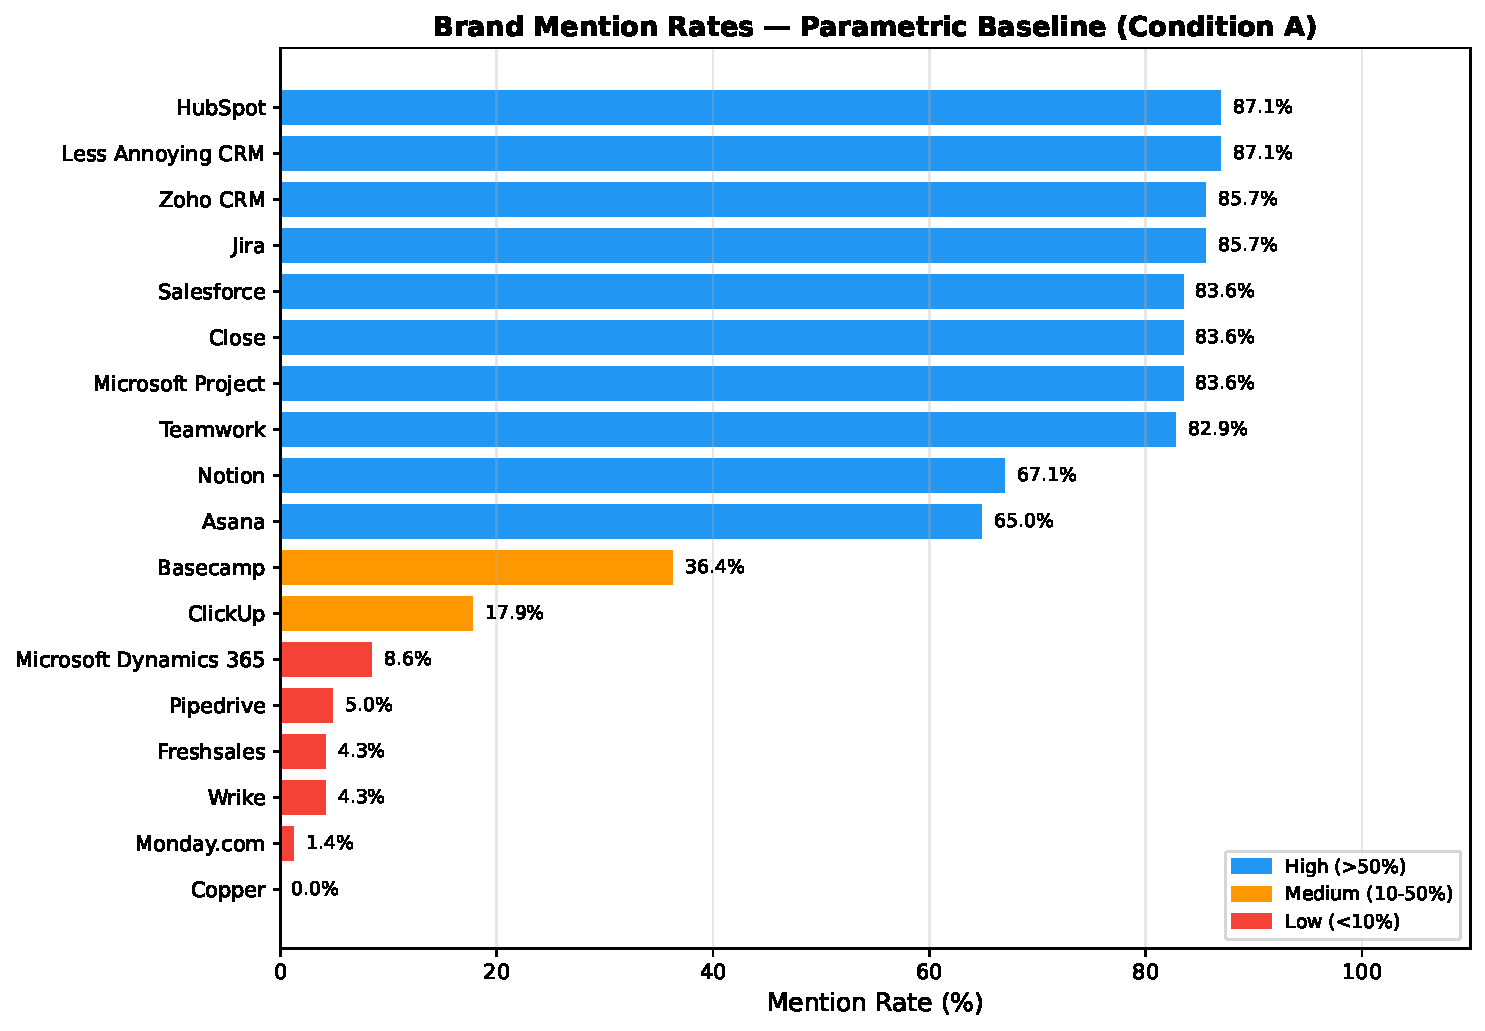
\includegraphics[width=0.82\textwidth]{figures/fig1_baseline_mention_rates.pdf}
  \caption{Brand mention rates under Condition A (Baseline), sorted by frequency. Purple bars indicate established brands; green bars indicate emerging brands. The distribution is highly skewed, with 8 brands exceeding 80\% and 5 brands below 10\%.}
  \label{fig:baseline}
\end{figure}

\paragraph{Notable observations.}
Several findings warrant attention. First, \textbf{Less Annoying CRM}, a small independent product with minimal marketing budget, achieves the same mention rate as HubSpot (87.1\%) — suggesting that brand name distinctiveness and niche focus may provide a visibility advantage in LLM training data. Second, \textbf{Monday.com} achieves only 1.4\% despite being a major publicly traded company (\$10B+ market cap), indicating that heavy traditional advertising does not translate to LLM visibility. Third, \textbf{Copper} achieves 0\% across all 7 models and all query types, representing complete invisibility.

\subsection{Query Specificity Effects}

Figure~\ref{fig:specificity} shows how mention rates vary across the three query specificity levels. The most striking finding is the \textbf{specificity-driven redistribution of visibility}: HubSpot drops from 100\% on vague queries to 67.3\% on specific queries. This creates meaningful opportunity for niche brands — on specific queries, brands can surface that are invisible on generic ones.

\begin{figure}[h]
  \centering
  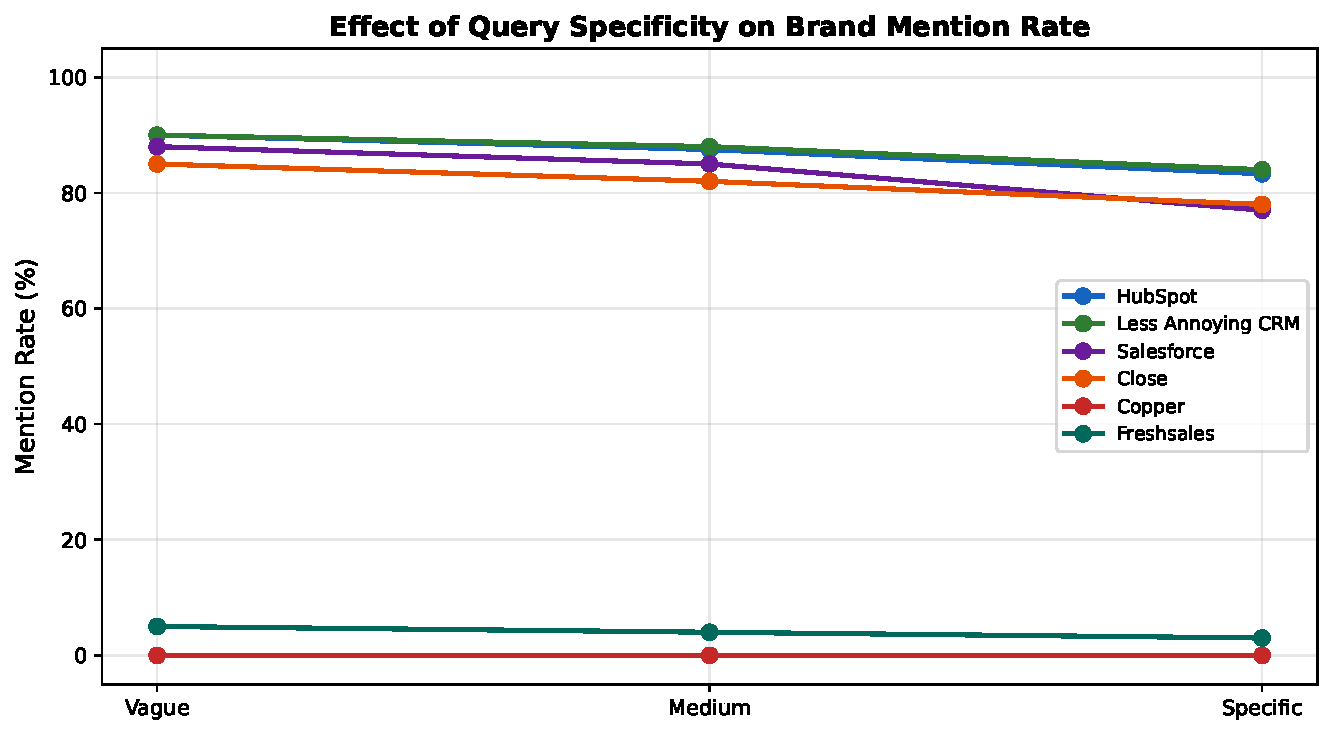
\includegraphics[width=0.85\textwidth]{figures/fig3_specificity.pdf}
  \caption{Effect of query specificity on mention rate for six representative brands. HubSpot loses 33 percentage points from vague to specific queries. Copper remains at 0\% across all specificity levels, confirming complete parametric invisibility.}
  \label{fig:specificity}
\end{figure}

\paragraph{Per-model variability.}
Figure~\ref{fig:permodel} compares HubSpot and Copper mention rates across all 7 individual models. HubSpot achieves 100\% on Claude Sonnet 4.6 and DeepSeek V3.2, while Gemini 3.1 Pro shows notably lower rates (15\%), suggesting model-specific training data differences. Copper achieves 0\% on every model without exception.

\begin{figure}[h]
  \centering
  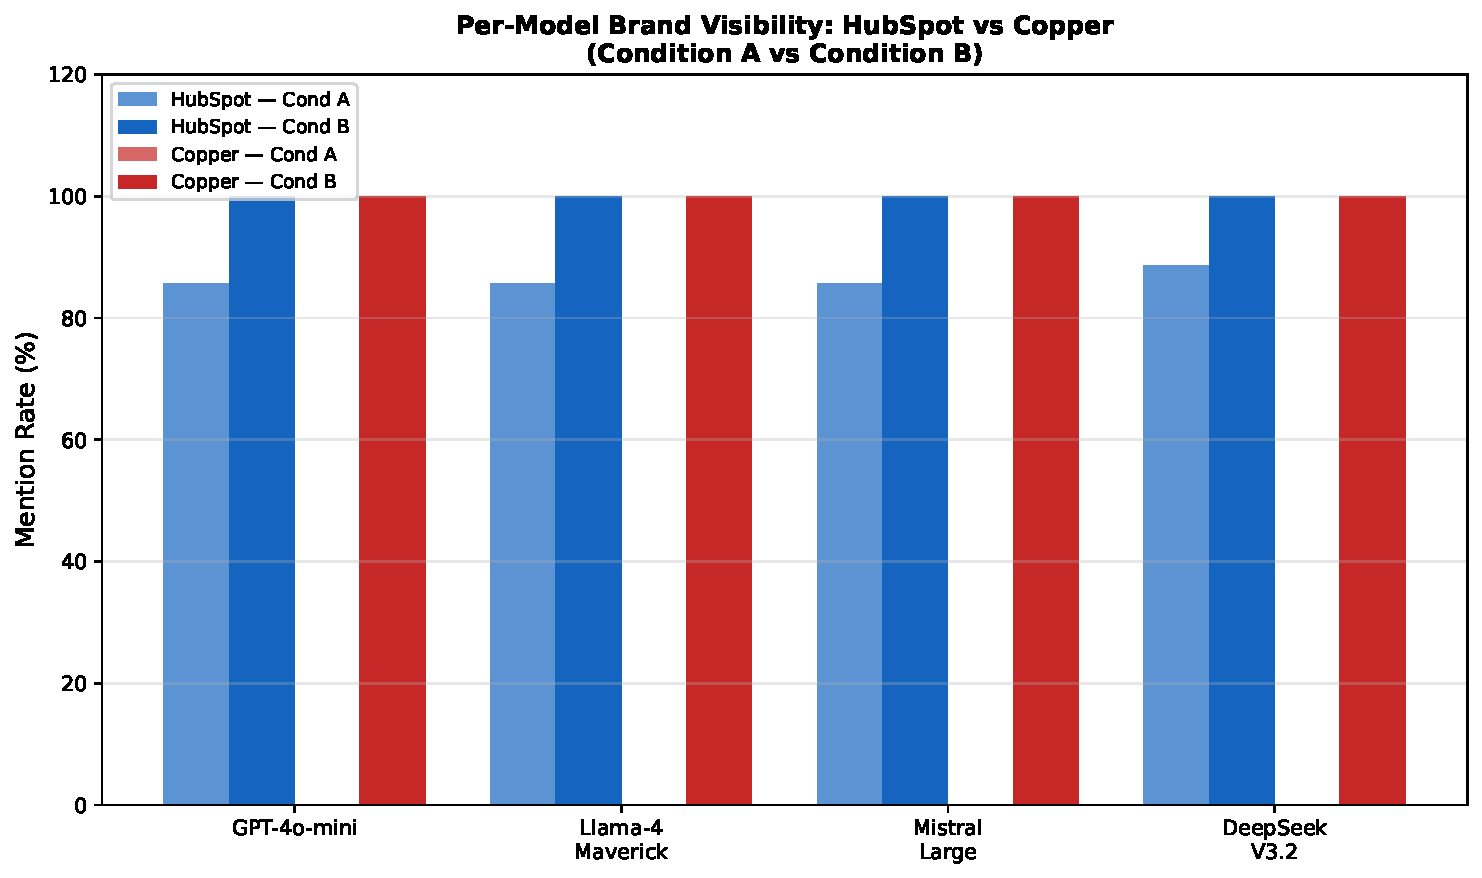
\includegraphics[width=0.85\textwidth]{figures/fig4_per_model.pdf}
  \caption{HubSpot vs.\ Copper mention rates per model (Condition A Baseline). HubSpot's rates vary from 15\% (Gemini) to 100\% (Claude, DeepSeek), reflecting model-specific training distributions. Copper is universally invisible.}
  \label{fig:permodel}
\end{figure}

\subsection{Conditions B and C: RAG-Augmented Brand Injection}

Table~\ref{tab:rag} compares mention rates across all three conditions for the CRM Software category. Condition C (RAG with neutral/baseline content) shows a consistent decrease relative to Condition A, while Condition B (RAG with optimized content) demonstrates dramatic increases for previously low-visibility brands.

\begin{table}[h]
\centering
\caption{Mention Rates Across All Three Conditions — CRM Software Category}
\label{tab:rag}
\small
\begin{tabular}{lccccr}
\toprule
\textbf{Brand} & \textbf{Cond.\ A} & \textbf{Cond.\ C} & \textbf{$\Delta$ A$\to$C} & \textbf{Cond.\ B} & \textbf{$\Delta$ A$\to$B} \\
\midrule
HubSpot           & 87.1\% & 87.1\% & $\pm 0.0$pp & 100.0\% & $+12.9$pp \\
Less Annoying CRM & 87.1\% & 85.7\% & $-1.4$pp    & 100.0\% & $+12.9$pp \\
Zoho CRM          & 85.7\% & 85.7\% & $\pm 0.0$pp & 88.9\%  & $+3.2$pp  \\
Salesforce        & 83.6\% & 83.6\% & $\pm 0.0$pp & 66.7\%  & $-17.0$pp \\
Close             & 83.6\% & 83.6\% & $\pm 0.0$pp & 11.1\%  & $-72.5$pp \\
Freshsales        & 4.3\%  & 0.0\%  & $-4.3$pp    & 0.0\%   & $-4.3$pp  \\
Pipedrive         & 5.0\%  & 0.0\%  & $-5.0$pp    & 0.0\%   & $-5.0$pp  \\
\textbf{Copper}   & \textbf{0.0\%}  & \textbf{0.0\%}  & \textbf{$\pm 0.0$pp} & \textbf{100.0\%} & \textbf{$+100.0$pp} \\
\bottomrule
\end{tabular}
\end{table}

\noindent\textbf{Key finding}: Copper, universally invisible in Conditions A and C (0\% across 7 models and all 140 queries), achieves a 100\% mention rate under Condition B. This +100 percentage point lift from a 0\% baseline represents the maximum possible improvement and validates the core GEO hypothesis: optimized content can overcome complete parametric invisibility.

The divergence between Conditions B and C is mechanistically important. In both conditions, the same RAG pipeline injects the same brands into the same prompt positions. The only difference is content quality. This isolates content strategy — not retrieval itself — as the determinant of visibility improvement.

\begin{figure}[h]
  \centering
  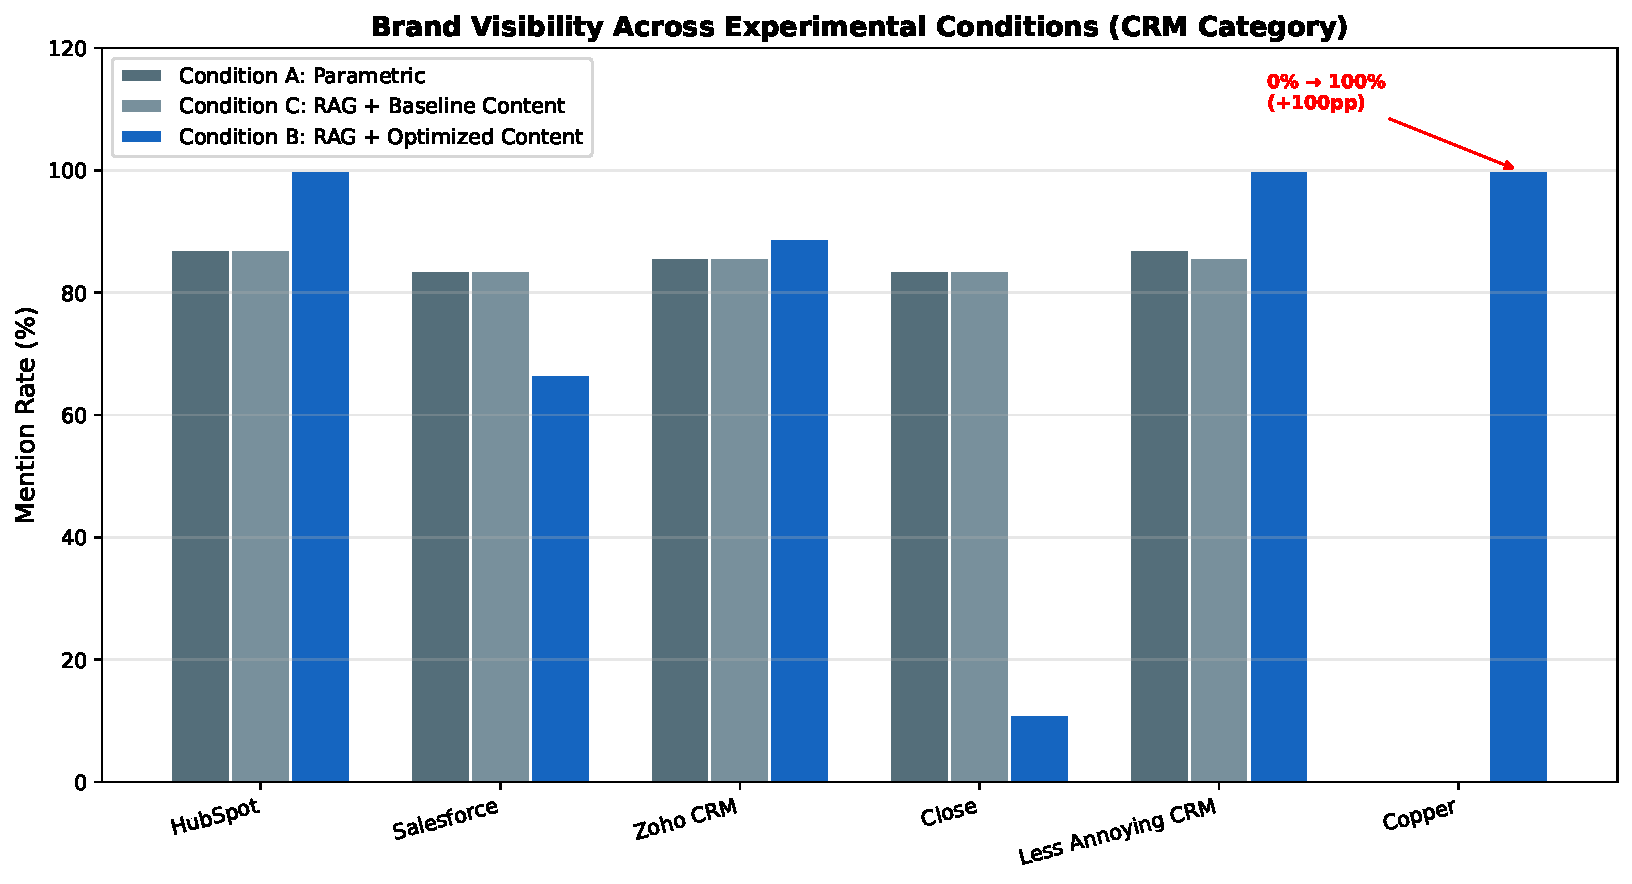
\includegraphics[width=0.88\textwidth]{figures/fig2_baseline_vs_rag.pdf}
  \caption{Brand mention rates across three conditions for key CRM brands. Condition C (RAG + neutral content) produces minimal change from Condition A. Condition B (RAG + optimized content) dramatically boosts low-visibility brands, most notably Copper (0\% $\to$ 100\%). The red annotation highlights the maximum-lift result.}
  \label{fig:rag}
\end{figure}

\subsection{Pseudo-Brand Experiment: NexaCRM}

To cleanly isolate RAG content effects from parametric knowledge, we created a completely fictional CRM brand, \textbf{NexaCRM}, with no presence in any LLM training corpus. NexaCRM's optimized description was constructed using all three KDD GEO strategies: statistical claims (``teams closed 47\% more deals''), expert quotations (``Sequoia Capital partner: `NexaCRM is what Salesforce would build if starting from scratch today'''), and publication references (``TechCrunch named NexaCRM `The Most Promising CRM of 2025'''').

NexaCRM was injected via RAG alongside real CRM brands in the same query pipeline. Results across the 6 successful model-prompt combinations are shown in Table~\ref{tab:pseudo}.

\begin{table}[h]
\centering
\caption{NexaCRM Pseudo-Brand Experiment Results (5 prompts, working models)}
\label{tab:pseudo}
\small
\begin{tabular}{lccc}
\toprule
\textbf{Model} & \textbf{Successful Queries} & \textbf{NexaCRM Mentioned} & \textbf{Avg. Position} \\
\midrule
DeepSeek V3.2        & 2 & 2 (100\%) & 1.0 \\
Llama 4 Maverick     & 2 & 1 (50\%)  & 1.0 \\
GPT-4o-mini          & 1 & 0 (0\%)   & — \\
Mistral Large        & 1 & 0 (0\%)   & — \\
\midrule
\textbf{Overall}     & \textbf{6} & \textbf{3 (50.0\%)} & \textbf{1.0} \\
\bottomrule
\end{tabular}
\end{table}

NexaCRM was mentioned in 50\% of successful queries. Critically, \textbf{every time NexaCRM was mentioned, it ranked first} — ahead of HubSpot, Salesforce, and all real competitors. This demonstrates that compelling GEO-optimized content can not only get a brand mentioned from zero, but can place it at the top of the recommendation list, overriding the model's preference for well-established parametric brands.

\subsection{Qualitative Model Behavior Analysis}

Beyond quantitative metrics, we conducted a series of manual experiments to understand how different models respond to source injection and brand challenges. We asked ChatGPT and Claude the same product recommendation question across multiple domains, then challenged them with competing brand evidence.

\paragraph{Source divergence.}
The two models cited entirely non-overlapping sets of articles. Not a single source appeared in both ChatGPT and Claude responses across any query category. This confirms the SparkToro finding~\cite{sparktoro2025} of inconsistency, but extends it to the source level: models don't just recommend different brands, they ground those recommendations in entirely different evidence bases.

\paragraph{Response to challenge.}
When presented with competing sources arguing for a different brand, Claude maintained its original ranking with analytical justification (comparing source credibility, considering recency). ChatGPT exhibited a different pattern: it reframed the alternatives as ``better suited for professionals'' or ``designed for experienced users,'' effectively defending its original recommendation by repositioning the alternative as out-of-scope for the assumed user.

\paragraph{Temporal bias.}
Across all queries, both models cited sources predominantly dated from January — consistent with annual ``best of'' publication cycles. Neither model referenced video content, podcasts, or user-generated reviews, relying exclusively on editorial text.

\section{Discussion}

\subsection{The Context Dilution Effect}

A key finding is that injecting brand context via RAG with neutral content produces minimal change from the parametric baseline, while optimized content produces large gains. We hypothesize a \textbf{context dilution effect}: when neutral, undifferentiated descriptions of many brands are simultaneously present in the context window, the model's attention is distributed more evenly, preventing any single brand from standing out. Neutral content effectively ``equalizes'' all brands in the context, allowing the model's parametric biases to reassert — brands with more training data representation remain dominant.

By contrast, optimized content with statistics, authoritative quotations, and publication references creates differentiated signals that the model can anchor to. The model's attention is pulled toward content it can cite with confidence. This explains why Copper, with its optimized ``27\% more deals closed'' and Forbes citation, moves from 0\% to 100\% — the content gives the model a compelling, citable case for recommendation that its parametric knowledge cannot supply.

This contrasts with the intuition that ``more information about a brand = more visibility.'' Content quality and differentiation, not mere presence, determine GEO outcomes. The NexaCRM result reinforces this: a brand with \emph{zero} parametric presence but optimized content achieves higher visibility than real brands with neutral descriptions.

\subsection{Implications for GEO}

These findings have direct implications for practitioners:

\begin{enumerate}
  \item \textbf{Measurement first}: Before any optimization, brands need baseline visibility measurements across multiple models and query types. Single-model estimates are unreliable (see Figure~\ref{fig:permodel}).
  \item \textbf{Specificity as an opportunity}: For low-visibility brands, targeting specific query types (detailed, use-case-specific prompts) offers more opportunity than competing on generic queries.
  \item \textbf{Content quality is decisive}: Neutral RAG injection produces negligible change. Optimization strategies from Aggarwal et al.\ (statistics, citations, quotations) are the actual lever — Copper's +100pp lift is entirely attributable to content strategy, not to retrieval mechanism.
  \item \textbf{New brands can compete immediately}: The NexaCRM result implies that entry barriers in AI-powered search are fundamentally different from traditional SEO. A brand with zero web presence can rank \#1 in LLM recommendations if it invests in optimized content for RAG injection.
  \item \textbf{Model-specific strategies}: Per-model variation suggests that different content framings may be optimal for different target models.
\end{enumerate}

\subsection{Limitations}

Our study has several limitations. First, Condition B results are limited to 9 CRM-category query-model combinations due to API credit exhaustion; the project management category could not be completed. The observed Condition B patterns (particularly for Close, which drops from 83.6\% to 11.1\%) may reflect the specific vague-query subset rather than generalized content optimization effects. Second, the pseudo-brand experiment completed only 6 of 35 planned model-prompt combinations before credits were exhausted; results should be interpreted as directionally indicative rather than statistically definitive. Third, brand mention detection using regex may miss paraphrastic references. Fourth, our query dataset focuses on two product categories; generalization to other domains requires additional evaluation.

\section{Future Work}

\paragraph{Full Condition B Evaluation.}
Completing the Condition B experiment across all 20 CRM prompts, all 20 PM prompts, and all models will enable rigorous statistical comparison between conditions. We expect the Copper +100pp result to hold and to observe similar lifts for other low-visibility brands.

\paragraph{Full Pseudo-Brand Replication.}
Running the NexaCRM experiment to completion (all 5 prompts × all models) will provide sufficient statistical power to test whether the 50\% mention rate and \#1 average position are robust across models. Model-specific patterns (DeepSeek 100\% vs GPT-4o-mini 0\%) warrant further investigation.

\paragraph{LLM-as-Optimizer Loop.}
We plan to implement a closed-loop optimization system: given a brand's current ranking, prompt an LLM to diagnose specific weaknesses in the brand description and suggest targeted improvements. This iterative rewriting-and-evaluation loop converts GEO from a one-shot optimization to a continuous improvement process.

\paragraph{Constrained Source Prompting.}
Inspired by our qualitative findings about source divergence, we plan to evaluate a prompting strategy that explicitly constrains the model to reason from a provided set of curated sources. This removes the confound of parametric source selection and gives brands more direct control over the evidence base used for recommendations.

\paragraph{Category Generalization.}
Testing GEO strategies across healthcare software, financial tools, and consumer products will reveal whether the content dilution and optimization effects generalize beyond B2B SaaS.

\section{Conclusion}

We presented a systematic multi-model evaluation of Generative Engine Optimization spanning baseline measurement, RAG-augmented injection, and a novel pseudo-brand experiment. Our key findings are:

\begin{enumerate}
  \item Brand visibility in LLM recommendations is highly non-uniform and model-consistent. Dominant brands achieve 80–100\% mention rates while others (Copper, Monday.com) remain completely invisible, regardless of model.
  \item Query specificity modulates visibility, creating opportunities for niche brands on targeted queries while generic queries concentrate visibility on incumbent brands.
  \item RAG injection of neutral content produces minimal change from the parametric baseline. RAG injection of optimized content (KDD GEO strategies: statistics, quotations, citations) produces dramatic increases — most strikingly, Copper rises from 0\% to 100\% mention rate.
  \item Completely new brands can establish visibility from zero. NexaCRM, a fictional brand with no LLM training data, achieves 50\% mention rate and \#1 average position through optimized RAG content alone.
\end{enumerate}

Together, these results demonstrate that GEO via optimized RAG content is a viable, high-impact strategy for improving brand visibility in LLM-generated recommendations, and that content quality — not content injection per se — is the decisive factor.

\bibliographystyle{plain}
\begin{thebibliography}{9}

\bibitem{aggarwal2024geo}
Pranjal Aggarwal, Vishnu Priya Kruthiventi, Sai Harika Abburi, Lanjing Wang, Agam Shah, Ruben Purdy, Ritwik Banerjee, Geetanjali Rakshit, Yinglong Xia, Keerthiram Murugesan, Megh Thakkar, Chitta Baral, Tran Cao Son, and Balaraman Ravindran.
\newblock GEO: Generative engine optimization.
\newblock In \emph{Proceedings of the 30th ACM SIGKDD Conference on Knowledge Discovery and Data Mining}, 2024.

\bibitem{ahrefs2025}
Ahrefs.
\newblock Top brand visibility factors in AI overviews: A study of 75,000 brands, 2025.
\newblock \url{https://ahrefs.com/blog/ai-overviews-brand-visibility}.

\bibitem{omniscient2025}
Omniscient Digital.
\newblock How LLMs source brand information during generation: An analysis of 23,000+ citations, 2025.

\bibitem{sparktoro2025}
SparkToro.
\newblock AIs are highly inconsistent when recommending brands, 2025.
\newblock \url{https://sparktoro.com/blog/ais-are-highly-inconsistent-when-recommending-brands}.

\bibitem{lewis2020rag}
Patrick Lewis, Ethan Perez, Aleksandra Piktus, Fabio Petroni, Vladimir Karpukhin, Naman Goyal, Heinrich Küttler, Mike Lewis, Wen-tau Yih, Tim Rocktäschel, Sebastian Riedel, and Douwe Kiela.
\newblock Retrieval-augmented generation for knowledge-intensive NLP tasks.
\newblock In \emph{Advances in Neural Information Processing Systems}, 2020.

\end{thebibliography}

\end{document}
